\newpage
\setcounter{secnumdepth}{3}
\section{Programming: REINFORCE on CartPole [12 pts]}

In this programming task you will implement \textbf{REINFORCE}, the basic policy
gradient algorithm, in PyTorch, and use it to train an agent to balance a pole on
a moving cart. This programming section is worth 37 points: 25 points for the
autograder and 12 points for the empirical questions in Section~\ref{sec:rl-empirical}.

\textbf{Important Note on PyTorch:} In this task you are REQUIRED to
use the automatic differentiation in PyTorch. You are allowed to use the built-in
neural network modules in PyTorch (such as \verb|nn.Linear|, \verb|nn.ReLU|,
\verb|nn.Sequential|, etc.) unless otherwise specified.

\textbf{PyTorch modules that are NOT allowed in this task:}
\begin{enumerate}
    \item \verb|torch.distributions| (e.g.\ \verb|torch.distributions.Categorical|).
    Sample actions using \verb|torch.multinomial| instead, as described below.
\end{enumerate}

\subsection{Setup}

We recommend creating a fresh conda environment for this assignment:

\begin{lstlisting}[language=Shell]
$ conda env create -f environment.yml
$ conda activate 10701-env-hw5
\end{lstlisting}

Alternatively, \verb|pip install -r requirements.txt| into an existing environment.
The only new dependency relative to previous assignments is
\href{https://gymnasium.farama.org/}{\texttt{gymnasium}}, a standard library of
reinforcement learning environments.

\subsection{The CartPole Environment}

\begin{center}
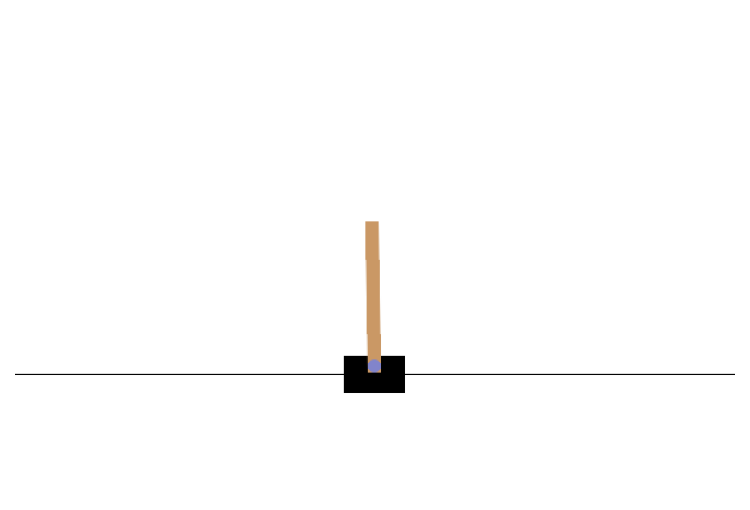
\includegraphics[height=4cm]{figures/cartpole.png}
\end{center}

A pole is attached by an unactuated joint to a cart that slides along a
frictionless track. The pole starts upright, and the agent's job is to keep it
from falling over by pushing the cart left or right.

\begin{itemize}
    \item \textbf{State.} A vector $s_t \in \Rb^4$ containing the cart position,
    the cart velocity, the pole angle, and the pole angular velocity.
    \item \textbf{Actions.} Two discrete actions: $0$ pushes the cart left and
    $1$ pushes the cart right. The agent must push one way or the other at
    every timestep; doing nothing is not an option.
    \item \textbf{Reward.} $+1$ for every timestep the pole remains upright,
    including the timestep on which the episode ends. \textbf{Note that every
    reward is positive} -- we will return to this fact in
    Section~\ref{sec:baseline}, where it turns out to matter a great deal.
    \item \textbf{Episode end.} An episode ends in one of two ways. It
    \emph{terminates} when the agent fails: the pole tips more than
    $12^{\circ}$ from vertical, or the cart runs off the end of the track. It is
    \emph{truncated} when it reaches \verb|max_steps|, the cap we place on
    episode length. Truncation is not a failure -- the agent was doing fine and
    we simply stopped watching.
\end{itemize}

Since the agent collects $+1$ per surviving step, the undiscounted return of an
episode is exactly the number of steps it lasted, and the best achievable return
is \verb|max_steps|. This makes the return easy to interpret: a return of $200$
with \verb|max_steps=200| means a perfect episode.

We provide the environment in \texttt{environment.py} as a thin wrapper around
Gymnasium's \verb|CartPole-v1|. \textbf{Please read this file carefully before
you start.} It exposes two methods:

\begin{itemize}
    \item \verb|reset(seed=None)|: Resets the environment and returns the
    initial state as a \verb|float32| tensor of shape $(4,)$. \textbf{Pass a seed
    only once per program}, which we already do for you in \verb|main|. Seeding
    before every episode would make every episode start from an identical state
    and learning would break.

    \item \verb|step(action)|: Takes action $0$ or $1$ and returns the tuple
    $(\texttt{state}, \texttt{reward}, \texttt{terminated}, \texttt{truncated})$.
    If \emph{either} \verb|terminated| or \verb|truncated| is \verb|True| the
    episode is over and you must stop collecting the trajectory.
\end{itemize}

\subsection{The REINFORCE Algorithm}

We want to learn a stochastic policy $\pi_\theta(a \mid s)$: a distribution over
actions, represented by a neural network with parameters $\theta \in \mathbb{R}^d$.
As discussed in lecture, running the policy produces a trajectory
$\tau = (s_1, a_1, r_1, \dots, s_T, a_T, r_T)$, and our objective is the expected
total discounted reward:
\begin{equation}
    J(\theta) = \Eb_{\pi_\theta}\left[ r_1 + \gamma r_2 + \gamma^2 r_3 + \cdots + \gamma^{T-1} r_T \right].
\end{equation}

We would like to do gradient \emph{ascent} on $J(\theta)$, but $J$ is an
expectation over trajectories whose distribution itself depends on $\theta$, so
we cannot simply differentiate inside the expectation. The \textbf{policy gradient
theorem} from lecture gives us a way around this. Given a sampled trajectory,
define for each step $t$
\begin{align}
    \label{eq:returns}
    A_t &= \sum_{i=t}^{T} \gamma^{\,i-t} r_i
         = r_t + \gamma r_{t+1} + \cdots + \gamma^{T-t} r_T
         && \text{(empirical total reward starting from step $t$)}, \\
    u_t &= \frac{d}{d\theta} \ln \pi_\theta(a_t \mid s_t) \in \mathbb{R}^d
         && \text{(action score vector, from autodiff)},
\end{align}
and the gradient estimate
\begin{equation}
    \label{eq:pg}
    g = \sum_{t=1}^{T} A_t \, u_t \in \mathbb{R}^d.
\end{equation}
For $\gamma = 1$, the theorem says $g$ is an unbiased estimate of
$\frac{dJ}{d\theta}$, even though we know nothing about the environment. For
$\gamma < 1$, the exact gradient would also weight step $t$ by $\gamma^{t-1}$,
which comes from the discounted visitation frequency $d^\pi(s)$ in the policy
gradient theorem. As discussed in lecture, we drop this factor. This is standard practice: it makes $g$ a
slightly biased estimate, but it works well and keeps the algorithm simple.

For equation~\ref{eq:pg}, the score vector $u_t$ is the
parameter direction that would increase the (log-)probability of taking action
$a_t$ in state $s_t$. Scaling it by $A_t$ upweights the score vector when the
reward that followed was large, and flips it if $A_t$ is negative. On average,
$g$ changes the policy to take actions more often if they were associated with
high total future reward.

\textbf{REINFORCE} simply uses $g$ as the gradient in an SGD-like update. In code
we do not form $g$ directly; instead we write down a loss whose derivative is
proportional to $-g$, since PyTorch optimizers \emph{minimize}:
\begin{equation}
    \label{eq:loss}
    \mathcal{L}(\theta) = -\frac{1}{T}\sum_{t=1}^{T} A_t \ln \pi_\theta(a_t \mid s_t),
    \qquad \text{so that} \qquad
    \frac{d\mathcal{L}}{d\theta} = -\frac{1}{T}\, g.
\end{equation}
Calling \verb|.backward()| on Equation~\ref{eq:loss} and stepping the optimizer
performs one step of gradient ascent on $J(\theta)$.

\subsubsection{Batching episodes}
\label{sec:batching}
A single trajectory gives a very noisy estimate of
the gradient. To reduce that noise we collect $M$ = \verb|episodes_per_update|
trajectories $\tau^1, \dots, \tau^M$ (as in lecture, the superscript $m$ indexes
the trajectory) and average their gradient estimates $g^1, \dots, g^M$. To do
this, call \verb|.backward()| on each trajectory's loss (divided by
\verb|episodes_per_update|, so that we accumulate an average rather than a sum),
and only then take a single optimizer step. PyTorch accumulates gradients across
\verb|.backward()| calls by default, which is exactly what we want here.
\textbf{This means you must zero the gradients only \emph{after} stepping the
optimizer, never between the episodes of a batch.}

\subsection{Reducing Variance with a Baseline}
\label{sec:baseline}

The estimate $g$ is unbiased (up to the discounting choice above), but it has
very high variance, and on CartPole it has a specific pathology. Every reward is
$+1$, so $A_t > 0$ at \emph{every} step of \emph{every} trajectory. Look at what
the update then does: it multiplies the score vector $u_t$ by a positive number
for every action the agent took, which pushes up the probability of
\emph{every} action it tried, good or bad. Learning happens only because good
actions get a \emph{larger} positive push than bad ones; the signal is carried
entirely by the relative sizes of the $A_t$, and it is swamped by their shared
offset.

The fix, as in lecture, is to subtract a \textbf{baseline}. Here we use a simple
one: the trajectory's mean return $\mu = \frac{1}{T}\sum_{t=1}^{T} A_t$,
subtracted from every $A_t$. You might reasonably object that changing the loss
should change what we optimize. It does not. Recall the argument from lecture:
since $\sum_a \pi_\theta(a \mid s) = 1$ for every state $s$, differentiating both
sides gives $\sum_a \frac{d}{d\theta} \pi_\theta(a \mid s) = 0$, and using the
log identity,
\begin{equation}
    \Eb_{a \sim \pi_\theta}\left[ \frac{d}{d\theta} \ln \pi_\theta(a \mid s) \right]
    = \sum_a \pi_\theta(a \mid s) \, \frac{d}{d\theta} \ln \pi_\theta(a \mid s)
    = \sum_a \frac{d}{d\theta} \pi_\theta(a \mid s) = 0.
\end{equation}
So for \emph{any} quantity $b$ that does not depend on the action $a_t$, the term
$b \, u_t$ is zero on average: any per-state offset to $A_t$ cancels out, and
subtracting it leaves the expected gradient untouched while changing the
variance.\footnote{Strictly, $\mu$ is computed from the same trajectory that
produced $a_t$, so it is only approximately independent of it. The resulting
bias is $O(1/T)$, and using a sample mean as a baseline is standard practice.}

We also divide by the standard deviation
$\sigma = \sqrt{\frac{1}{T}\sum_{t=1}^{T} (A_t - \mu)^2}$, which keeps the scale of
the updates roughly constant as the agent improves:
\begin{equation}
    \label{eq:standardize}
    \hat{A}_t = \frac{A_t - \mu}{\sigma + \epsilon}.
\end{equation}
Note that this rescaling is \emph{not} covered by the argument above: it scales
the gradient rather than shifting it, and is best understood as an adaptive step
size rather than a baseline. Using $\hat{A}_t$ in place of $A_t$ gives the loss
you will actually implement:
\begin{equation}
    \label{eq:loss-standardized}
    \mathcal{L}(\theta) = -\frac{1}{T}\sum_{t=1}^{T} \hat{A}_t \ln \pi_\theta(a_t \mid s_t).
\end{equation}
Now roughly half the $\hat{A}_t$ are negative, so the score vectors of
worse-than-average actions are flipped: those actions are actively pushed
\emph{down}.

You will implement this as \texttt{standardize\_returns}, controlled by the
\texttt{standardize} argument of \texttt{main}, so that you can run with it on
and off and measure the difference yourself.

\subsection{File Structure}

The handout contains the following files:

\begin{itemize}
    \item \texttt{reinforce.py}: The file in which you will implement REINFORCE.
    \textbf{This is the only file you submit.}
    \item \texttt{environment.py}: The CartPole environment (provided).
    \item \texttt{utils.py}: Plotting helpers (provided).
    \item \texttt{check.py}, \texttt{check\_data.pkl}: Local self-tests (provided).
    \item \texttt{requirements.txt}, \texttt{environment.yml}: Dependencies.
\end{itemize}

\subsection{Implementation Details}

You will implement the following in \texttt{reinforce.py}, in this order. Each is
marked with a \verb|# TODO:| comment in the starter code. Train your agent using
the hyperparameters specified in the starter code.

\begin{itemize}

    \item \texttt{PolicyNetwork}: A PyTorch module mapping a state to one logit
    per action. Use exactly two hidden linear layers of size \verb|hidden_size|
    with ReLU in between; any other architecture will fail the autograder. Keep
    the layer names in the provided \verb|nn.Sequential(OrderedDict([...]))|
    unchanged, as the self-tests load reference weights by name. Output
    \textbf{logits, not probabilities}: applying a softmax here and a logarithm
    later is numerically unstable for large logits.

    \item \texttt{get\_action}: Samples an action from the policy at a given
    state, using \verb|torch.nn.functional.softmax| and \verb|torch.multinomial|.
    We \emph{sample} rather than take the \verb|argmax| -- the randomness is what
    makes the agent explore, and what makes the policy gradient well defined.
    Wrap it in \verb|torch.no_grad()| and return a Python \verb|int|.

    \item \texttt{collect\_episode}: Runs the policy in the environment for one
    episode. Mind the shapes and dtypes in the docstring: \verb|states| is
    \verb|float32| $(T, 4)$, \verb|actions| is \verb|int64| $(T,)$, and
    \verb|rewards| is \verb|float32| $(T,)$. Store the state the action was taken
    \emph{from}, and remember that \emph{both} \verb|terminated| and
    \verb|truncated| end the episode.

    \item \texttt{discounted\_returns}: Computes $A_t$ at every timestep
    (Equation~\ref{eq:returns}). Since $A_t = r_t + \gamma A_{t+1}$, working
    backwards from the last timestep gives every $A_t$ in a single pass; you
    never need a nested loop.

    \item \texttt{standardize\_returns}: Standardizes one episode's returns
    (Equation~\ref{eq:standardize}). Add $\epsilon = 10^{-8}$ to the denominator:
    if the returns are all identical the standard deviation is zero, and
    dividing by it yields \texttt{nan} and silently destroys your policy.

    \item \texttt{policy\_loss}: Computes the REINFORCE loss
    (Equation~\ref{eq:loss}) and must return a \textbf{scalar} tensor.\\
    Use
    \verb|torch.nn.functional.log_softmax| for $\ln \pi_\theta(a_t \mid s_t)$
    for stability, and \verb|torch.gather| to
    pick out the action actually taken. The same code works for raw $A_t$ and
    standardized $\hat{A}_t$, which is why
    Equation~\ref{eq:loss-standardized} needs no separate implementation.

    \item \texttt{shape\_rewards}: \textbf{Provided, and returns the environment
    rewards unchanged.} \texttt{train} passes its rewards through this function
    before computing returns, so that the agent's learning signal can be changed
    without touching anything else. You do not need to modify it until
    Empirical Question 2.

    \item \texttt{train}: Performs one policy update from a batch of episodes.
    Call \verb|.backward()| on each episode's loss, then take \emph{one}
    optimizer step and zero the gradients \emph{afterwards}. Do not zero them
    inside the loop: accumulating across the batch is the averaging described in
    Section~\ref{sec:batching}.

    \item \texttt{evaluate}: Measures the mean undiscounted return of the current
    policy over \verb|eval_episodes| episodes, without updating it. The policy
    stays stochastic -- sample actions exactly as during training.

    \item \texttt{run}: The outer training loop. Calls \texttt{train}
    \verb|num_updates| times, runs \texttt{evaluate} every \verb|eval_every|
    updates, and returns both histories for plotting.

    \item \texttt{main}: Initializes the environment, the policy network, and the
    optimizer (use Adam). The environment is seeded once here; do not re-seed it
    anywhere else.

\end{itemize}

\subsection{Running the Agent}

\begin{lstlisting}[language=Shell]
$ python reinforce.py
\end{lstlisting}

Training with the default hyperparameters takes about a minute on a CPU.
The program saves a plot of the training and evaluation returns to
\texttt{training\_returns.png} and prints the final evaluation return. A correct
implementation should show the evaluation return climbing from roughly $20$ to
close to the maximum of $200$.

To change a hyperparameter, edit the defaults of \verb|main| or call it directly.

\subsection{Testing}

We provide self-tests for the individual functions you implement:

\begin{lstlisting}[language=Shell]
$ python check.py
\end{lstlisting}

Each check is independent and supplies its own inputs, so a later check passing
does \textbf{not} mean an earlier component is correct. Work through failures from
the top down. Note that passing every check does not test your training loop end
to end -- you still need to run \verb|reinforce.py| and confirm that your agent
actually learns.

\subsection{Empirical Questions}
\label{sec:rl-empirical}

\begin{enumerate}
    \item \textbf{[4 pts]} Train your agent with the default hyperparameters and
    include the resulting plot of training and evaluation returns below. Report
    the final evaluation return.

    \begin{tcolorbox}[fit,height=10cm, width=15cm, blank, borderline={1pt}{-2pt}]
        %%% Write your solution here %%%

    \end{tcolorbox}

    \clearpage

    \item \textbf{[8 pts]} \textbf{Designing a better reward.}
    CartPole's native reward is $+1$ for every timestep survived, so the
    undiscounted return is just the number of steps the pole stayed up. That is
    the quantity we genuinely care about, but it is not necessarily the most
    useful \emph{learning signal}: it says nothing about whether the pole is
    comfortably upright or a hair away from falling, until it is too late.

    You will design a replacement. Edit the body of \texttt{shape\_rewards} in
    \texttt{reinforce.py}, which receives the episode's states and environment
    rewards and returns the rewards the agent should \emph{learn} from. For
    example, you might reward the agent only while the pole is within a few
    degrees of vertical, or scale the reward smoothly with the tilt angle, or
    penalise drifting away from the centre of the track.

    \textbf{Everything reported still uses the true environment reward.} Your
    shaped reward changes only what the agent learns from, never how it is
    scored, so you cannot improve your numbers by simply handing out more
    reward. Make sure you understand why this distinction is essential before
    you start: a shaped reward that scores well on itself but survives fewer
    steps has made the agent worse, not better.

    \textbf{How we measure it.} With the default hyperparameters, both the original
    reward and a good shaped reward end up near $200$, so the final return
    cannot tell them apart. What a better learning signal buys us is
    \emph{training speed}. We therefore measure the \textbf{number of policy updates
    needed to reach a return of $195$}, defined as the first evaluation at which
    the return reaches $195$ \emph{and stays at or above it for the next
    evaluation too} -- a single lucky evaluation does not count. Lower is better.

    \texttt{main} returns \verb|(train_returns, eval_returns)|, and
    \verb|eval_returns[i]| is the evaluation after\\
    $(i+1) \times$
    \verb|eval_every| updates, so you can read this number straight off that
    list.

    \textbf{What to report.}
    \begin{enumerate}[label=(\alph*)]
        \item The reward function you designed, as a formula or a few lines of
        code, and one sentence on the intuition behind it.
        \item A comparison against the unmodified reward. Run \textbf{both} the
        default \texttt{shape\_rewards} and your version on the \textbf{same
        five seeds} $\{10702,\ 10704,\ 10720,\ 10724,\ 10729\}$, and fill in the
        table below with the updates-to-$195$ from each run.
        \item Two or three sentences explaining \emph{why} your reward helped or
        hurt, in terms of the learning signal it provides. If your \textbf{mean}
        is not lower than the default's mean, explain what you think went wrong.
        Note that single seeds are noisy: a reward that performs well on three seeds and
        bad on two has still probably helped, which is why we compare means
        over five.
    \end{enumerate}

    \begin{center}
    \begin{tabular}{lcccccc}
    \toprule
    \multicolumn{7}{c}{\emph{policy updates needed to reach a return of 195 (lower is better)}} \\
    reward & 10702 & 10704 & 10720 & 10724 & 10729 & mean \\
    \midrule
    default ($+1$ per step) & & & & & & \\
    yours                   & & & & & & \\
    \bottomrule
    \end{tabular}
    \end{center}

    \begin{tcolorbox}[fit,height=13cm, width=15cm, blank, borderline={1pt}{-2pt}]
        %%% Write your solution here %%%

    \end{tcolorbox}

\end{enumerate}
